Заключительный алгоритм, который будет рассмотрен в рамках способов поиска миностовов -- алгоритм Буровки.

\section{Мысли о реализации}

Изначально будем считать, что у нас есть $|V|$ тривиальных деревьев из одной вершины.

Будем пытаться эти деревья расширять, соединяя между собой. 
Звучит достаточно логично, что на каждом шаге дерево $T_1$ соединить с таким деревом $T_2$, что ребро, которое их соединяет, будет минимально по весу (которое и войдёт в миностов).

Но у такой схемы есть явная проблема. Тут могут появиться циклы, а миностов, как мы помним, это дерево. Вот пример ситуации.

\begin{figure}[H]
    \centering
    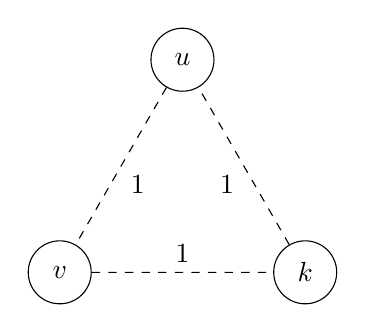
\begin{tikzpicture}[scale=1.5]
        \tikzstyle{vertex}=[circle, draw, minimum size=0.8cm, inner sep=0pt]

        \node[vertex] (u) at (90:1.2) {$u$};
        \node[vertex] (v) at (210:1.2) {$v$};
        \node[vertex] (k) at (330:1.2) {$k$};

        \draw[dashed] (u) -- node[auto] {1} (v);
        \draw[dashed] (v) -- node[auto] {1} (k);
        \draw[dashed] (k) -- node[auto] {1} (u);
    \end{tikzpicture}    
\end{figure}

Здесь, $u, v, k$ вершины в начале алгоритма -- <<тривиальные деревья>>. Между вершинами по ребру весом 1. После итерации алгоритма мы выберем минимальные рёбра, которые мы добавим в миностов. 
Потенциально могло произойти следующее:
\begin{enumerate}
    \item Для $u$: ребро $(u, v)$.
    \item Для $v$: ребро $(v, k)$.
    \item Для $k$: ребро $(k, v)$.
\end{enumerate}
Так произошло в силу того, что каждое ребро одинакового веса и все они минимальны. Поэтому получается такая картина.


\begin{figure}[H]
    \centering
    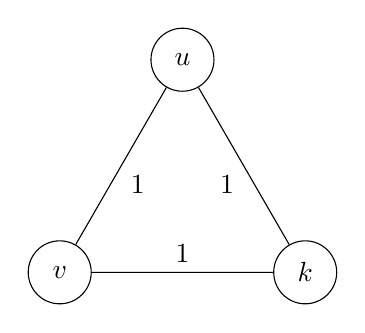
\begin{tikzpicture}[scale=1.5]
        \tikzstyle{vertex}=[circle, draw, minimum size=0.8cm, inner sep=0pt]

        \node[vertex] (u) at (90:1.2) {$u$};
        \node[vertex] (v) at (210:1.2) {$v$};
        \node[vertex] (k) at (330:1.2) {$k$};

        \draw (u) -- node[auto] {1} (v);
        \draw (v) -- node[auto] {1} (k);
        \draw (k) -- node[auto] {1} (u);
    \end{tikzpicture}    
\end{figure}

Получили цикл, чего быть, очевидно, не должно.

Чтобы устранить циклы, предлагается пронумеровать все вершины. \textit{И если минимальных рёбер несколько, то выбирать с минимальным номером.}

Тогда воспроизведём прошлый пример с некоторой нумерацией.

\begin{figure}[H]
    \centering
    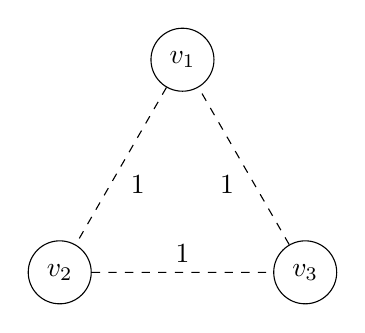
\begin{tikzpicture}[scale=1.5]
        \tikzstyle{vertex}=[circle, draw, minimum size=0.8cm, inner sep=0pt]

        \node[vertex] (u) at (90:1.2) {$v_1$};
        \node[vertex] (v) at (210:1.2) {$v_2$};
        \node[vertex] (k) at (330:1.2) {$v_3$};

        \draw[dashed] (u) -- node[auto] {1} (v);
        \draw[dashed] (v) -- node[auto] {1} (k);
        \draw[dashed] (k) -- node[auto] {1} (u);
    \end{tikzpicture}    
\end{figure}

Тогда будут выбраны следующие рёбра:
\begin{enumerate}
    \item Для $v_1$: $(v_1, v_2)$.
    \item Для $v_2$: $(v_2, v_1)$.
    \item Для $v_3$: $(v_3, v_1)$.
\end{enumerate}
И тогда уже получится слудующая картина:

\begin{figure}[H]
    \centering
    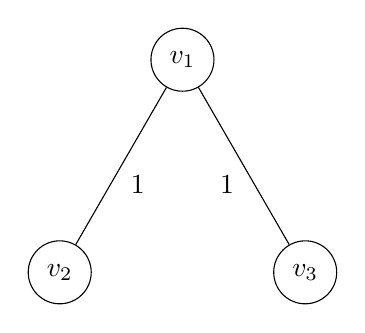
\begin{tikzpicture}[scale=1.5]
        \tikzstyle{vertex}=[circle, draw, minimum size=0.8cm, inner sep=0pt]

        \node[vertex] (u) at (90:1.2) {$v_1$};
        \node[vertex] (v) at (210:1.2) {$v_2$};
        \node[vertex] (k) at (330:1.2) {$v_3$};

        \draw (u) -- node[auto] {1} (v);
        \draw (k) -- node[auto] {1} (u);
    \end{tikzpicture}    
\end{figure}

Как можно видеть, циклов нет. Позже мы покажем формально, что циклов действительно не будет в общем случае.

\section{Алгоритм}

Рассмотрим теперь сам алгоритм. Будем считать, что каждая вершина имеет поле \texttt{t}, которое повзоляет определить порядковый номер дерева, в котором оно лежит.
Порядковый номер выставляется с помощью метода \texttt{DFS\_COMP}, который просто запускает \texttt{DFS}, нумерующий компоненты связности (деревья).
Читателю предлагается, самому придумать реализацию \texttt{DFS\_COMP}, в силу её тривиальности. Очевидно, что она работает за $\O(|V| + |E|)$.
Также у вершины есть поле $\texttt{n}$ -- порядковый номер вершины. Метод, который нумерует вершины графа $G$ будем обозначать \texttt{NUM\_GRAPH}. 
Очевидно, его можно реализовать, чтобы он работал за $\Theta(|V|)$.

Далее считаем, что $w(\varnothing) = +\infty$.

\begin{algorithm}[H]
\caption{Алгоритм Борувки}
\begin{algorithmic}[1]

\Function{BORUVKA}{$G\langle V, E \rangle, w$}
    \State $\texttt{NUM\_GRAPH(}G\texttt{)}$
    \State $T \gets []$

    \While{$|T| < |V| - 1$} \Comment{Пока у нас не осталось одно единственное дерево -- миностов}
        \State $e_m \gets \{\}$ \Comment{Будем хранить минимальные рёбра для деревьев}
        
        \State $\texttt{DFS\_COMP}(T)$

        \For{$(u, v) \in E$}
            \If{$u\texttt{.t} \neq v\texttt{.t}$} \Comment{Вершины лежат в разных дервьях}
                \If{$w(e_m[u\texttt{.t}]) > w(u, v) \lor w(e_m[u\texttt{.t}]) = w(u, v) \land (\text{$v$ имеет меньший номер})$}
                    \State $e_m[u\texttt{.t}] \gets (u, v)$
                \EndIf

                \If{$w(e_m[v\texttt{.t}]) > w(u, v) \lor w(e_m[v\texttt{.t}]) = w(u, v) \land (\text{$u$ имеет меньший номер})$}
                    \State $e_m[v\texttt{.t}] \gets (u, v)$
                \EndIf
            \EndIf
        \EndFor

        \For{$(t, e) \in e_m$} \Comment{Проходимся по деревьям, чтобы их расширить рёбрами}
            \State $T\texttt{.ADD\_EDGE(}e\texttt{)}$
        \EndFor
    \EndWhile

    \State \Return $T$
\EndFunction
\end{algorithmic}
\end{algorithm}

\Exe Подумайте, как можно убрать \texttt{DFS} и лишнее поле $\texttt{t}$ внутри \texttt{while} с помощью СНМ. 

\St Функция \texttt{BORUVKA} работает за $\O(|E| \log |V|)$.
\begin{proof}

    Каждую итерацию, количество деревьев уменьшается хотя бы в два раза. Действительно, каждой компоненте связности мы ищем по ребру, которое связывает её с другой компонентой, а значит как минимум две компоненты объединяются в одну.
    Значит, итераций цикла $\O(\log |V|)$. Далее, $\texttt{DFS\_COMP}$ работает за $\O(|E|)$ и цикл на 7-ой строке тоже за $\O(|E|)$. Значит суммарное время работы $\O(|E| \log |V|)$.

\end{proof}

\section{Корректность}

Для начала покажем, что граф, который возвращается, всё-таки ацикличен. В рамках этой части надо ввести одно специфичное определение для доказательства утверждения ацикличности.

\Def Графом $T_n\langle V_{T_n}, E_{T_n} \rangle$ будем называть \textit{ориентированный граф}, который был получен на $n$-ой итерации цикла к моменту 13-ой строчки алгоритма \texttt{BORUVKA}, следующим способом. 
Вершины в нём будут компоненты связности $t_1, t_2, \dots t_p$ (деревья), которые были в $T$ на $n$-ой итерации цикла. 
А множество рёбер определяется взятием каждой комнентой связности и проведением \textit{из} неё \textit{в ту}, в которое идёт минимальное по весу ребро полученное на строчках 10, либо 12.

\Note Заметим, что по сути вершинами графа $T_n$ являются компоненты связности $T$ на момент $n$-ой интерации. Поэтому далее мы будем отождествлять вершины $T_n$ с компонентами связности $T$.

\Note $T_n$ необязательно слабо связный граф. Вполне может быть несколько компонент слабой связности.

Возьмём наш пример, который мы привели в самом начале.

\begin{figure}[H]
    \centering
    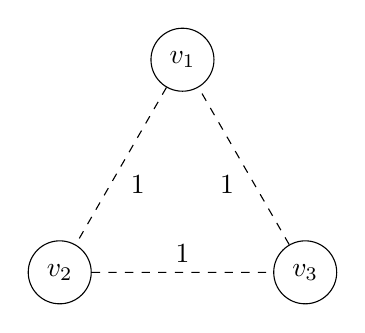
\begin{tikzpicture}[scale=1.5]
        \tikzstyle{vertex}=[circle, draw, minimum size=0.8cm, inner sep=0pt]

        \node[vertex] (u) at (90:1.2) {$v_1$};
        \node[vertex] (v) at (210:1.2) {$v_2$};
        \node[vertex] (k) at (330:1.2) {$v_3$};

        \draw[dashed] (u) -- node[auto] {1} (v);
        \draw[dashed] (v) -- node[auto] {1} (k);
        \draw[dashed] (k) -- node[auto] {1} (u);
    \end{tikzpicture}    
\end{figure}

Тогда $T_1$ будет представлять собой:
\begin{figure}[H]
    \centering
    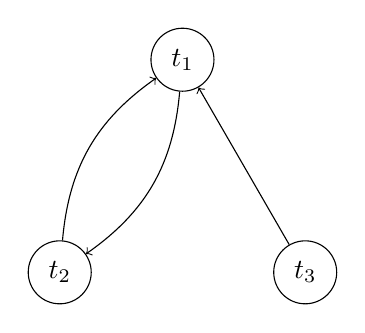
\begin{tikzpicture}[scale=1.5]
        \tikzstyle{vertex}=[circle, draw, minimum size=0.8cm, inner sep=0pt]

        \node[vertex] (u) at (90:1.2) {$t_1$};
        \node[vertex] (v) at (210:1.2) {$t_2$};
        \node[vertex] (k) at (330:1.2) {$t_3$};

        \draw[->, bend left=25] (u) to (v);
        \draw[->, bend left=25] (v) to (u);
        \draw[->] (k) -- (u);;
    \end{tikzpicture}    
\end{figure}

Ведь:
\begin{enumerate}
    \item Для $v_1$ (компонента связности $t_1$): $(v_1, v_2)$.
    \item Для $v_2$ (компонента связности $t_2$): $(v_2, v_1)$.
    \item Для $v_3$ (компонента связности $t_3$): $(v_3, v_1)$.
\end{enumerate}

\Note Заметим, что в графе $T_1$ есть циклы длины 2, но по факту это одно и то же ребро $(v_1, v_2)$, ведь исходный граф неориентированный. На самом деле утверждается, что циклов длины более чем 2 не существует в таком графе.

\Def Функциональным графом будем называть граф, у которого из каждой вершины исходит ровно одно ребро.

\St $\forall n \hookrightarrow \text{$T_n$ -- функциональный граф}$.
\begin{proof}
    
    Действительно, мы для каждой компоненты связности находим ровно одно ребро, которое мы потом ориентируем от него, в строчках 10 либо 12.

\end{proof}

Далее, если для ребра $e$ графа $T_n$, мы пишем $w(e)$, то мы имеем в виду вес соотвествующего ребра оригинального графа.

\St Если в графе $T_n$ есть рёбра $(t_i, t_j)$ и $(t_j, t_k)$, то $w(t_i, t_j) \geq w(t_j, t_k)$. Более того, если $w(t_i, t_j) = w(t_j, t_k)$, то $k < i$.
\begin{proof}
    
    Если такие рёбра есть, то в строчках 10 либо 12 при рассмотрении вершины $t_j$ отдался приоритет вершине $t_k$, значит, вес ребра $(t_j, t_k)$ уж точно не больше, чем $(t_i, t_j)$.
    Но коль у нас произошло равенство весов, то в строчках 10 либо 12 рассматривался вторым приоритетом номер вершины и в силу того, что для $t_j$ выбралось $t_k$, то $t_k$ имело меньший номер, чем $t_i \Rightarrow i > j$.

\end{proof}

\St $\forall n \hookrightarrow \text{$T_n$ не содержит циклов длины более 2}$.
\begin{proof}
    
    Предположим противное, что содержит. Значит, есть цикл $t_1 \to t_2 \to \dots \to t_c \to t_1$. По утверждению выше, получаем следующую цепочку неравенств:
    \begin{equation*}
        w(t_1, t_2) \leq w(t_2, t_3) \leq \dots \leq w(t_{c - 1}, t_c) \leq w(t_c, t_1) \leq w(t_1, t_2)
    \end{equation*}
    Значит:
    \begin{equation*}
        w(t_1, t_2) = w(t_2, t_3) = \dots = w(t_{c - 1}, t_c) = w(t_c, t_1)
    \end{equation*} 
    
    Рассмотрим случаи и воспользуемся всё тем же утверждением.

    \begin{enumerate}
        \item $c = 2p + 1$, т.е. $c$ -- нечётное
            \begin{equation*}
                t_1 > t_3 > \dots > t_{2p + 1} > t_2 > t_4 > \dots t_{2p} > t_1
            \end{equation*}
            Противоречие
        \item $c = 2p$, т.е. $c$ -- чётное
            \begin{equation*}
                t_1 > t_3 > \dots > t_{2p - 1} > t_1
            \end{equation*}
            Противоречие
    \end{enumerate}

\end{proof}

\Cons $\forall n \hookrightarrow$ Каждая компонента слабой связности $T_n$ содержит ровно один цикл длины 2.
\begin{proof}
    
    Вспомним, что $T_n$ -- функциональный. В частности любая компнента слабой связности $T_n$, очевидно, функциональный граф. Также легко видеть, что хотя бы один цикл есть. По утверждению выше, они все длины 2.

    Предположим, что циклов длины 2 хотя бы 2 штуки: $t_i \to t_j \to t_i$ и $t_k \to t_l \to t_k$. Тогда заметим, что, по определению, функционального графа из вершин $t_i, t_j, t_k, t_l$ не выходит ни одного ребра в остальные вершины слабой КС, а значит пришли к противоречию.

\end{proof}

Доказательство следующего утверждения изложено достаточно формально в общем случае и может показаться достаточно сложным. 
Но на самом деле здесь описаны те же самые действия, которые происходили на оригинальной лекции, только более подробно и на экзамене прямо так как написано тут необязательно.
Читателю предлагается ориентироваться на это доказательство в первую очередь, если у него возникли какие-то вопросы к доказательству с лекции или он хочет очень детально его разобрать. 
Далее в начале мы приведём менее формальное, но достаточно понятное доказательство, которое было на лекции, а далее будет приведено формальное доказательство этого утверждения (которое автор очень просит \textit{не приводить на экзамене (!!!)} за полной бессмысленностью этого действия и потенциального страдания экзаменаторов).

Как говорил классик: \textit{<<Ваза опрокидывается>>}.

\St Функция \texttt{BORUVKA} возвращает миностов
\begin{proof}

    Граф $T_{n_0}$ распадется на несколько компонент слабой свзяности. Рассмотрим одну из них.

    Заметим, что по сути собой граф представляет собой <<дерево>>. Подвесим его за вершину $u$ такую, что она участвует в цикле длины 2, который единственный в функциональном подграфе.
    Далее доказательство будет приведено на примере, потому что в общем случае рассуждения аналогичны. Пусть компонента связности выглядит следующим образом:

    \begin{figure}[H]
        \centering
        \begin{tikzpicture}[scale=1.2, every node/.style={circle, draw, minimum size=0.7cm, inner sep=0pt}]
            \node (b) at (-3, -2) {$b$};
            \node (c) at (-1, -2) {$c$};
            \node (a) at (-2, 0) {$a$};
            \node (u) at (-2, 2) {$u$};

            \node (r) at (1, -2) {$r$};
            \node (l) at (3, -2) {$l$};
            \node (d) at (2, 0) {$d$};
            \node (v) at (2, 2) {$v$};

            \draw[-Stealth, thick] (b) -- (a);
            \draw[-Stealth, thick] (c) -- (a);
            \draw[-Stealth, thick] (a) -- (u);

            \draw[-Stealth, thick] (r) -- (d);
            \draw[-Stealth, thick] (l) -- (d);
            \draw[-Stealth, thick] (d) -- (v);

            \draw[-Stealth, thick, bend left=25] (u) to (v);
            \draw[-Stealth, thick, bend left=25] (v) to (u);
        \end{tikzpicture}
    \end{figure}
    
    Рассмотрим вершину $b$ и ребро $(b, a)$. Заметим, что ребро $(b, a)$ минимально по весу среди всех рёбер пересекающих разрез из одной вершины $b$ и всех остальных кроме неё.
    Поэтому, по лемме о безопасном ребре $(b, a)$ безопасное, поэтому можем добавить её в миностов.
    Такое же рассуждение проведём для вершины $c$ и ребра $(c, a)$. Далее осталось рассмотреть вершину $a$ и ребро $(a, u)$.
    Предположим, что $(u, a)$ не минимальное ребро среди тех, что пересекают разрез и \textit{строго меньше по весу}, чем $(u, a)$. Тогда существует некоторое ребро или из $b$, или из $c$, которое тоже пересекает разрез. Без потери общности будем считать, что это ребро $(b, u')$.

    В силу того, что алгоритмом было выбрано ребро $(b, a)$, значит, это ребро минимально по весу среди всех, что выходят из $b$. Значит верно:
    \begin{equation*}
        w(b, a) \leq w(b, u')
    \end{equation*}
    Далее, применим утверждение 5.3.8 к ребрам $(b, a)$ и $(a, u)$:
    \begin{equation*}
        w(a, u) \leq w(b, a)
    \end{equation*}
    Кобминируя два неравенства выше и предположение, получаем следующую цепочку:
    \begin{equation*}
        w(a, u) \leq w(b, a) \leq w(b, u') < w(a, u)
    \end{equation*}
    \begin{equation*}
        w(a, u) < w(a, u)
    \end{equation*}

    Противоречие. Значит, $(a, u)$ -- безопасное ребро, по лемме.

\end{proof}

И тот же классик говорил: \textit{<<Мне всё равно не нравилась эта ваза>>}.

\St Функция \texttt{BORUVKA} возвращает миностов
\begin{proof}
    
    Доказательство снова будет по индукции. Покажем, что на каждой итерации $T$ есть подграф некоторого миностова.

    База. Нулевая итерация (до начала цикла), тривиально, ведь там просто вершины без рёбер.

    Пусть $n_0 \geq 1$ и показали для $0, 1, \dots n_0 - 1$ итераций. Покажем для $n_0$ верность данного утверждения.

    Пусть к 13-ой строчке мы построили $T_{n_0}$. Далее мы будем добавлять рёбра из $T_{n_0}$ в $T$.

    Напомним, что вершинами в $T_{n_0}$ \textit{являются компоненты слабой связности} (т.е. деревья), которые образовались на момент $n_0$ итерации. 
    Поэтому, говоря о вершине $T_{n_0}$, мы будем иметь в виду, что данная вершина представляет собой множество вершин оригинального графа $G$, которые были объединены соответствующей компонентой слабой связности. 
    Также, когда мы будем говорить про рёбра $T_{n_0}$, мы будем иметь в виду в том числе соответствующие рёбра в \textit{оригинальном графе} $G$.

    Будем перебирать все компоненты слабой связности $T_{n_0}$. Рассмотрим конкретную компоненту $C$. По утверждению выше, $C$ имеет ровно один цикл длины 2, для определенности пусть он образован вершинами $u$ и $v$.
    Подвесим граф <<за цикл $(u, v)$>> и получим, например, такую картину:

    \begin{figure}[H]
        \centering
        \begin{tikzpicture}[scale=1.2, every node/.style={circle, draw, minimum size=0.7cm, inner sep=0pt}]
            \node (b) at (-3, -2) {$b$};
            \node (c) at (-1, -2) {$c$};
            \node (a) at (-2, 0) {$a$};
            \node (u) at (-2, 2) {$u$};

            \node (r) at (1, -2) {$r$};
            \node (l) at (3, -2) {$l$};
            \node (d) at (2, 0) {$d$};
            \node (v) at (2, 2) {$v$};

            \draw[-Stealth, thick] (b) -- (a);
            \draw[-Stealth, thick] (c) -- (a);
            \draw[-Stealth, thick] (a) -- (u);

            \draw[-Stealth, thick] (r) -- (d);
            \draw[-Stealth, thick] (l) -- (d);
            \draw[-Stealth, thick] (d) -- (v);

            \draw[-Stealth, thick, bend left=25] (u) to (v);
            \draw[-Stealth, thick, bend left=25] (v) to (u);
        \end{tikzpicture}
    \end{figure}

    Заметим, что если убрать $(u, v)$ и $(v, u)$, то мы получим два дерева. Вернём ребро $(v, u)$, тогда опять получим дерево. Подвесим его за вершину $u$.

    \begin{figure}[h]
            \centering
            \begin{tikzpicture}[
                scale=1.2, 
                every node/.style={circle, draw, minimum size=0.7cm, inner sep=0pt, font=\bfseries},
                level oval/.style={draw, dashed, thick, ellipse, inner sep=10pt}
            ]
                \node (b) at (-3, -2) {$b$};
                \node (c) at (-1, -2) {$c$};
                \node (r) at (1, -4) {$r$};
                \node (l) at (3, -4) {$l$};

                \node (a) at (-2, 0) {$a$};
                \node (d) at (2, -2) {$d$};

                \node (u) at (-2, 2) {$u$};
                \node (v) at (2, 0) {$v$};


                \draw[-Stealth, thick] (b) -- (a);
                \draw[-Stealth, thick] (c) -- (a);
                \draw[-Stealth, thick] (r) -- (d);
                \draw[-Stealth, thick] (l) -- (d);

                \draw[-Stealth, thick] (a) -- (u);
                \draw[-Stealth, thick] (d) -- (v);

                \draw[-Stealth, thick] (v) to (u);


                \node[level oval, fit=(r) (l), label={[font=\large, yshift=-5mm]left:3}] {};

                \node[level oval, fit=(b) (c) (d), label={[font=\large, yshift=5mm]left:2}] {};

                \node[level oval, fit=(a) (v), label={[font=\large, yshift=5mm]left:1}] {};

            \end{tikzpicture}
        \end{figure}

        Далее будем двигаться по глубине дерева снизу вверх, а по вершинам на одном уровне произвольно.
        
        Рассмотрим базу для самых глубоких вершин. Рассмотрим вершину $r$ и попытаемся добавить ребро $(r, d)$, которое из неё исходит. Пусть $(r, d)$ в оригинальном графе было $(v_r, v_d)$. Рассмотрим разрез $\mathcal{B} = (\{v_r, V \setminus \{v_r\}\})$. Тогда ясно, что $(v_r, v_d)$ -- минимальное ребро пересекающее разрез. Тогда по лемме о безопасном ребре, $T \cup \{ (v_r, v_d) \}$ -- подграф некоторого миностова. Считаем далее, что теперь в $T$ есть ребро $(v_r, v_d)$.
        Повторим итеративно для всех вершин на данном уровне эти же рассуждения.


        Для самого глубокого уровня показали, как базу индукции. Далее пусть мы рассмотрели все глубины большие $h$, рассмотрим вершины на глубине $h$.
        Возьмём вершину $b$. Возьмём её поддерево (в смысле в $T_{n_0}$). Заметим, что у дерева либо рёбер нет (как на картинке), либо рёбра уже были рассмотрены на предыдущих шагах (как например, у $d$ это рёбра $(r, d)$ и $(l, d)$).

        Пусть $V_b$ -- множество вершин, которые находятся в компонентах связности поддерева $b$, причем вершины из $b$ тоже принадлежат $V_b$. Рассмотрим разрез $\mathcal{B} = (V_b, V \setminus V_b)$. 
        Пусть $(b, a)$ было ребром $(v_b, v_a)$ в оригинальном графе.
        Заметим, что ребро (в смысле оригинального графа) $(v_b, v_a)$ -- минимальное по весу ребро, которое пересекает $\mathcal{B}$.
        Покажем же это. Разрез могут пересекать только лишь рёбра выходящие из $V_b$.
        Предположим, что такое есть и $(b, a)$ не минимально по весу. Пусть оно выходит из вершины $x \in V_b, x \not\in b$ ($x$ -- вершина графа $G$) и равно $(x, y)$, более того $w(x, y) < w(v_b, v_a)$. Также за $e$ обозначим ребро, которое выходило из компоненты связности, где лежал $x$ и было добавлено в миностов.

        Тогда:
        \begin{equation*}
            w(x, y) \geq w(e) \geq w(v_b, v_a)
        \end{equation*}
        Первое неравенство верно в силу того, что $e$ было выбрано при рассмотрении вершины $x$, а не $(x, y)$, а значит оно меньше по весу (см. строчки алгоритма 10 и 12). Второе неравенство обосновывается тем, что $e$ лежит на пути от компоненты связности, где лежит $x$, до $b$, а значит к нему можно применить итеративно по пути вышедоказанное утверждение 5.3.8.

        Но в тоже время, по предположению, заключаем:
        \begin{equation*}
            w(x, y) < w(v_b, v_a) \leq w(x, y)
        \end{equation*}
        \begin{equation*}
            w(x, y) < w(x, y)
        \end{equation*}
        Противоречие, такого ребра нет.

        Значит, опять можем воспользоваться леммой о безопасном ребре и получить при добавлении ребра $(v_b, v_a)$ подграф некоторого миностова. Далее считаем, что ребро добавлено.

        Проделав все рассуждения в указанном выше порядке, получим требуемое утвреждение.

\end{proof}
